\newpage
\section{Neuronale Netze}
Ein neuronales Netz ist ein Zusammenschluss aus mehreren Perceptronen in verschiedenen Layern. Als Beispiel sei an
dieser Stelle die Abbildung \ref{fig:07_neuronal_network} gegeben. Diese wird ebenso verwendet, um die Ableitungskette
für ein Gewicht in diesem Fall zu zeigen. Anzumerken sei hier, dass die Kombination der gewichteten Summen mit der
Aktivierungsfunktion ein Neuron darstellt.
\begin{figure}[h!]
    \begin{center}
        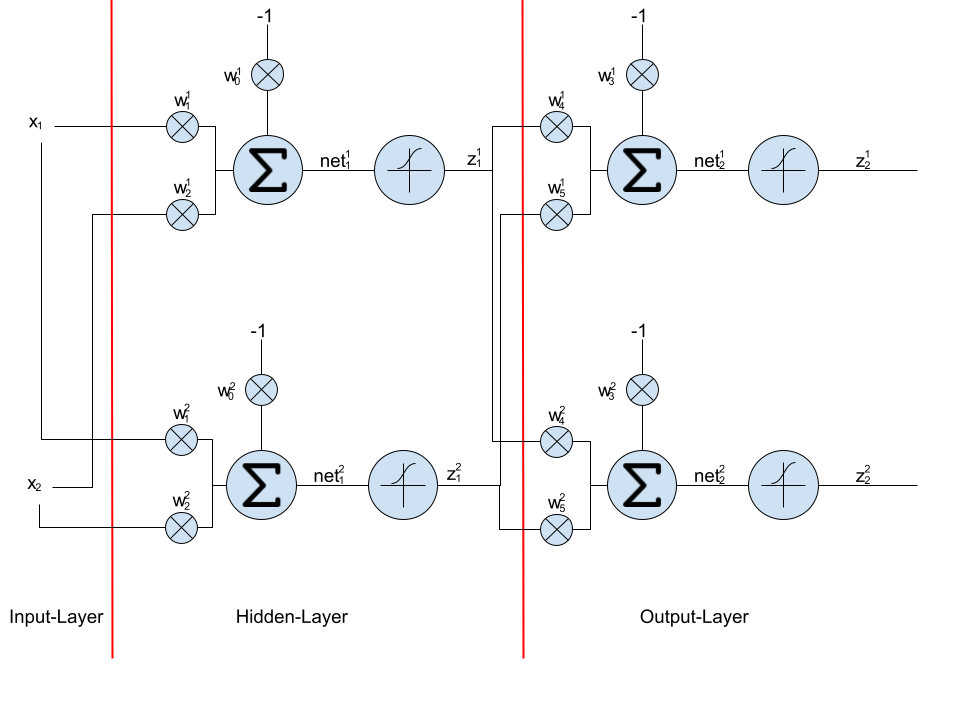
\includegraphics[width=1\linewidth]{../common/01_neuronal_network/00_resources/02_neuronales_netz.png}
    \end{center}
    \caption{Ein neuronales Netz mit einem Hidden-Layer}
    \label{fig:07_neuronal_network}
\end{figure}

\newpage
\subsection{Lernverfahren mit Gradientenabstieg}
Wie beim Perceptron auch soll nun an dieser Stelle die Komponente des Gradienten für das Gewicht $w_1^1$ gezeigt
werden. Für dieses Beispiel wird die Abbildung \ref{fig:08_neuronal_network} hinzugezogen.
\begin{figure}[h!]
    \begin{center}
        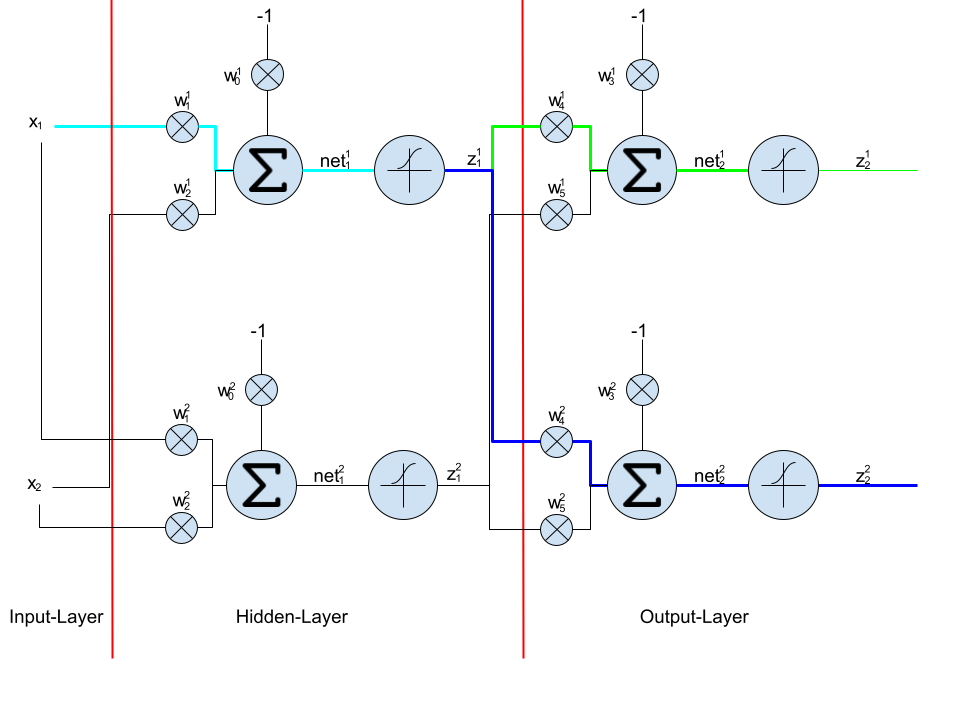
\includegraphics[width=1\linewidth]{../common/01_neuronal_network/00_resources/03_neuronales_netz_pfad.png}
    \end{center}
    \caption{Der Pfad zum Gewicht $w_1^1$ im neuronalen Netz}
    \label{fig:08_neuronal_network}
\end{figure}
Die Fehlerfunktion ist wie beim Perceptron dieselbe $P_{err} = - \frac{1}{2} \cdot \sum_i^2 (d^i - z_2^i)^2$.
In diesem Fall steht die Komponente $i$ für den Index und die $2$ für den Layer.
Zur Abbildung \ref{fig:08_neuronal_network} ist wichtig zu erkennen, dass für die Korrektor des Gewichts $w_1^1$
mehrere Wege relevant sind. Es kann einmal der grüne sowie der blaue Weg verfolgt werden. Der Teil, welcher bei
beiden gleich ist, wird cyan markiert.
Weiterhin sind folgende Werte sind bekannt:
\begin{align}
    P_{err} = - \frac{1}{2} \cdot \sum_i^2 (d^i - z_2^i)^2\\
    net_1^1 = x_1 \cdot w_1^1 + x_2 \cdot w_2^1 - w_0^1\\
    z_1^1 = \frac{1}{1 + e^{-net_1^1}}\\
    net_1^2 = x_1 \cdot w_1^2 + x_2 \cdot w_2^2 - w_0^2\\
    z_1^2 = \frac{1}{1 + e^{-net_1^2}}\\
    net_2^1 = z_1^1 \cdot w_4^1 + z_1^2 \cdot w_5^1 - w_3^1\\
    z_2^1 = \frac{1}{1 + e^{-net_2^1}}\\
    net_2^2 = z_1^1 \cdot w_4^2 + z_1^2 \cdot w_5^2 - w_3^2\\
    z_2^2 = \frac{1}{1 + e^{-net_2^2}}
\end{align}
Der Gradient für die Gewichte setzt sich wie nachfolgend zusammen:
\begin{align}
    \vec{\nabla} = (w_0^1, w_1^1, w_2^1, w_0^2, w_1^2, w_2^2, w_3^1, w_4^1, w_5^1, w_3^2, w_4^2, w_5^2)
\end{align}
Die Korrektur in einem Schritt kann wiederum über den Vektor der Gewichte $\vec{w}$ erfolgen.
\begin{align}
    \vec{w}_{neu} = \vec{w}_{alt} + \lambda \cdot \vec{\nabla}
\end{align}
Wie bereits erwähnt wird nur die Komponente $w_1^1$ aus dem Vektor $\vec{\nabla}$
berücksichtigt. Um diesen herzuleiten, müssen alle Pfade zum Gewicht berücksichtigt werden.
In dem Fall gibt es, wie in Abbildung \ref{fig:08_neuronal_network} entnommen werden kann, deren zwei.
Die Funktionskette ist in Gleichung \ref{eq:03_funktions_kette} ersichtlich. Es werden nur die wirklich relevanten Aufrufe
gezeigt.
\begin{multline}
    P_{err} = - \frac{1}{2} \cdot (d^1 - z_2^1(net_2^1(w_4^1 \cdot z_1^1(net_1^1(w_1^1 \cdot x_1, w_2^1 \cdot x_2, -w_0^1)), z_1^2 \cdot w_5^1, -w_3^1)))^2 +\\\label{eq:03_funktions_kette}
    - \frac{1}{2} \cdot (d^2 - z_2^2(net_2^2(w_4^2 \cdot z_1^1(net_1^1(w_1^1 \cdot x_1, w_2^1 \cdot x_2, -w_0^1)), z_1^2 \cdot w_5^2, -w_3^2)))^2
\end{multline}
Dementsprechend werden die beiden Pfade für die Komponente des Gradienten für $w_1^1$ berücksichtigt.
\begin{multline}
    \frac{\delta P_{err}}{\delta w_1^1} = \frac{\delta P_{err}}{\delta z_2^1(w_1^1)} \cdot \frac{\delta z_2^1(w_1^1)}{\delta net_2^1(w_1^1)} \cdot \frac{\delta net_2^1(w_1^1)}{\delta z_1^1(w_1^1)} \cdot \frac{\delta z_1^1(w_1^1)}{\delta net_1^1(w_1^1)} \cdot \frac{\delta net_1^1(w_1^1)}{\delta w_1^1} +\\
    \frac{\delta P_{err}}{\delta z_2^2(w_1^1)} \cdot \frac{\delta z_2^2(w_1^1)}{\delta net_2^2(w_1^1)} \cdot \frac{\delta net_2^2(w_1^1)}{\delta z_1^1(w_1^1)} \cdot \frac{\delta z_1^1(w_1^1)}{\delta net_1^1(w_1^1)} \cdot \frac{\delta net_1^1(w_1^1)}{\delta w_1^1}
\end{multline}
Anders ausgedrückt lautet demnach die Komponente:
\begin{multline}
    w_{1,korr}^1 = (d^1 - z_2^1) \cdot z_2^1(1 - z_2^1) \cdot w_4^1 \cdot z_1^1(1 - z_1^1) \cdot x_1 +\\
    (d^2 - z_2^2) \cdot z_2^2(1 - z_2^2) \cdot w_4^2 \cdot z_1^1(1 - z_1^1) \cdot x_1
\end{multline}
An dieser Stelle sei angemerkt, dass dieses Verfahren durchaus funktioniert, jedoch wachsen die Ableitungsterme
exponentiell mit der Anzahl Neuronen in den Layern. Aus diesem Grund ist der Gradientenabstieg so nicht brauchbar in
der Praxis. Was jedoch auffällt ist die Tatsache, dass einmal berechnete Ableitungsketten wiederverwendet werden können.
Gedanklich kann an dieser Stelle z.B. die Ableitungskette für $w_2^1$ hinzugezogen werden. Man erkennt relativ schnell,
dass viele Berechnung, welche schon für $w_1^1$ gemacht wurden, wiederauftreten. Auf Grundlage dieser Idee der
dynamischen Programmierung wurde der Backpropagation Algorithmus entwickelt.

\newpage
\subsection{Lernverfahren mit Backpropagation}
Der grosse Vorteil dieses Verfahrens ist die Berechnungszeit, welche im Vergleich zum reinen Gradientenabstieg nur noch
linear mit der Anzahl der Gewichte wächst. So werden einmal berechnete Ableitungsketten gespeichert und wiederverwendet.
Der Input-Layer wird nicht beachtet, dieser ist für die Berechnung irrelevant. Die verbleibenden Layer (Hidden-, Output-Layer)
bilden die zwei zu unterscheidenden Fälle des Algorithmus.
\\

Es folgen einige generelle Bemerkungen zu den Abbildungen \ref{fig:08_backpropagation_output} und \ref{fig:09_backpropagation_hidden}.
Der Algorithmus kann anhand eines neuronalen Netzes wie eine Schablone dreier Ebenen verstanden werden, die von rechts
nach links über die Layer des Netzwerks geschoben wird.
Es gibt eine blau markierte Ebene, diese ist dem aktuellen Berechnungsschritt von einem Vorausgehenden bereits bekannt.
Hier muss also nichts gemacht werden, diese Werte kennt man. Die grün markierte Ebene ist diejenige, welche im aktuellen
Berechnungsschritt für den Nächsten berechnet und auch gespeichert wird. Die orange markierte Ebene ist
die Korrektur der Gewichte im aktuellen Berechnungsschritt für den aktuellen Layer. In den jeweiligen Ebenen gibt
es eine relevante Stelle (als roter Pfeil markiert). Für jede Ebene hat diese Stelle eine gewisse Bedeutung. Bei der blauen Ebene markiert sie die
Position des Layers, bis zu welcher der Wert bekannt ist. Bei der grünen Ebene markiert sie das Resultat, welches berechnet
wird. Bei der orangen Ebene ist nur ein Beispiel für ein Gewicht gegeben. Auch dort wird das Resultat markiert, welches
berechnet wird (Ableitung der Fehlerfunktion nach einem spezifischen Gewicht zur Korrektur desselben). Diese Information
ist lediglich für den aktuellen Berechnungsschritt und Layer relevant und wird nicht gespeichert (das korrigierte Gewicht natürlich
schon). Als Beispiel ist ebenfalls eine Reihe von Neuronen ersichtlich, deren Indizes vollständig ausgeschrieben wurden.
Die untere Reihe wiederum befasst sich mit der verallgemeinert gültigen Schreibweise. Gewichte werden anhand der Neuronennummer
im Layer wie auch der Nummer des Gewichts innerhalb des Neurons indexiert. Für ein Gewicht $2$ im Neuron $3$ des Layers
$r$ lautet die Schreibweise demnach $w_{32}^r$.
\\

Beim ersten Fall des Algorithmus handelt es sich um den Output-Layer. Um dies zu veranschaulichen, kann
die Abbildung \ref{fig:08_backpropagation_output} betrachtet werden. In der blauen Ebene ist der Fehlerwert $P_{err}$
gegeben. Hierbei stehen die Angaben $r$ für die zu berechnende Schicht,
$i$ für die Anzahl der Neuronen der Schicht und $j$ für die Anzahl der Gewichte (Inputs), welche pro Neuron existieren.
Weiterhin gibt es die vorherige Schicht $p$, welche wiederum aus $s$ Neuronen besteht.
In diesem Beispiel ist $j = 3$. Die Gewichte erhalten dadurch mit $i = 2$ die folgende Nummerierung:
$w_{11}^r$, $w_{12}^r$, $w_{13}^r$, $w_{21}^r$, $w_{22}^r$, $w_{23}^r$. Ebenfalls relevant ist hierbei, dass es sich um ein \glqq fully connected
Network\grqq{} handelt, also alle jeweiligen Outputs mit allen Neuronen der folgenden Schicht verbunden sind.

\begin{figure}[h!]
    \begin{center}
        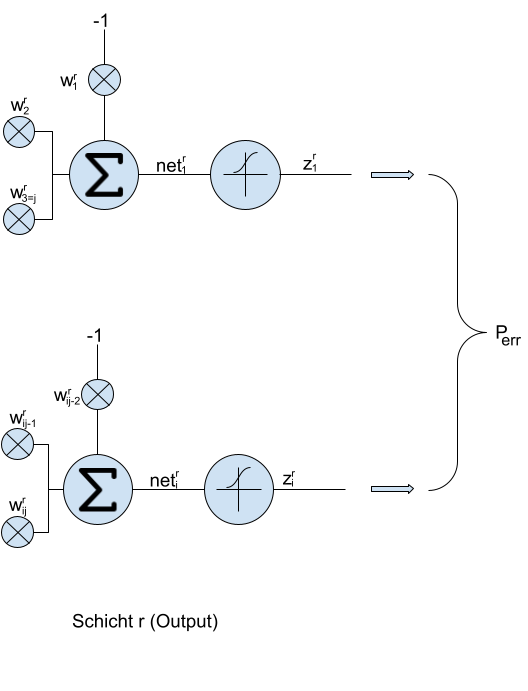
\includegraphics[width=1\linewidth]{../common/01_neuronal_network/00_resources/04_backpropagation_output.png}
    \end{center}
    \caption{Backpropagation für Output-Layer}
    \label{fig:08_backpropagation_output}
\end{figure}
Die grün markierte Ebene besteht nun aus der Berechnung des Terms $\delta_i^r$. Dieser Term beschreibt die Ableitungskette
$\frac{\delta P_{err}}{\delta net_i^r} = \frac{\delta P_{err}}{\delta z_i^r} \cdot \frac{\delta z_i^r}{\delta net_i^r}$.
Man beachte, dass es genau so viele Elemente $\delta_i^r$ wie Neuronen in der Schicht $r$ gibt.
Im Falle des Perceptrons gibt es z.B. nur ein Element, im Falle eines neuronalen Netzes gibt es im Output-Layer so viele Elemente wie
Output-Klassen (Neuronen).
Es kann also festgehalten werden, dass gilt:
\begin{align}
    \delta_i^r = (d_i^r - z_i^r) \cdot z_i^r(1 - z_i^r) \cdot \label{eq:04_delta_output}
\end{align}
Auf die orange markierte Ebene (Korrektur der Gewichte) wird nach der Erklärung des zweiten Falles eingegangen.

\newpage
Beim zweiten Fall handelt es sich um einen Hidden-Layer. Dazu kann Abbildung \ref{fig:09_backpropagation_hidden} hinzugezogen
werden. Wie vorhin auch steht hier $r$ für die Schicht, welche berechnet werden soll, $i$ für die Anzahl der Neuronen
der Schicht $r$, $j$ für die Anzahl der Gewichte (Inputs) pro Neuron der Schicht $r$, $k$ für die vorher berechnete
Schicht, $l$ für die Anzahl der Neuronen der Schicht $k$, $m$ für die Anzahl der Gewichte pro Neuron der Schicht $k$ (bei einem
\glqq fully connected Netzwerk\grqq{} gilt $m = i + 1$), $p$ für die vorherige Schicht, welche aus $s$ Neuronen besteht.
In der blauen Ebene der Abbildung können wiederum die bekannten Werte abgelesen werden.
Diese setzen sich aus den bereits vorhin gesehenen Termen\footnote{Anzumerken sei hier, dass es sich bei $l$ nur
um einen Platzhalter handelt. Die Nummerierung geht von $1$ bis $l$, es existieren also $l$ $\delta$.} $\delta_l^k$ zusammen. Es sind die Ableitungen der
Fehlerfunktion $P_{err}$ nach $net_l^k$. Wie bereits erwähnt gibt es so viele Terme, wie Neuronen der Schicht $k$.
\begin{figure}[h!]
    \begin{center}
        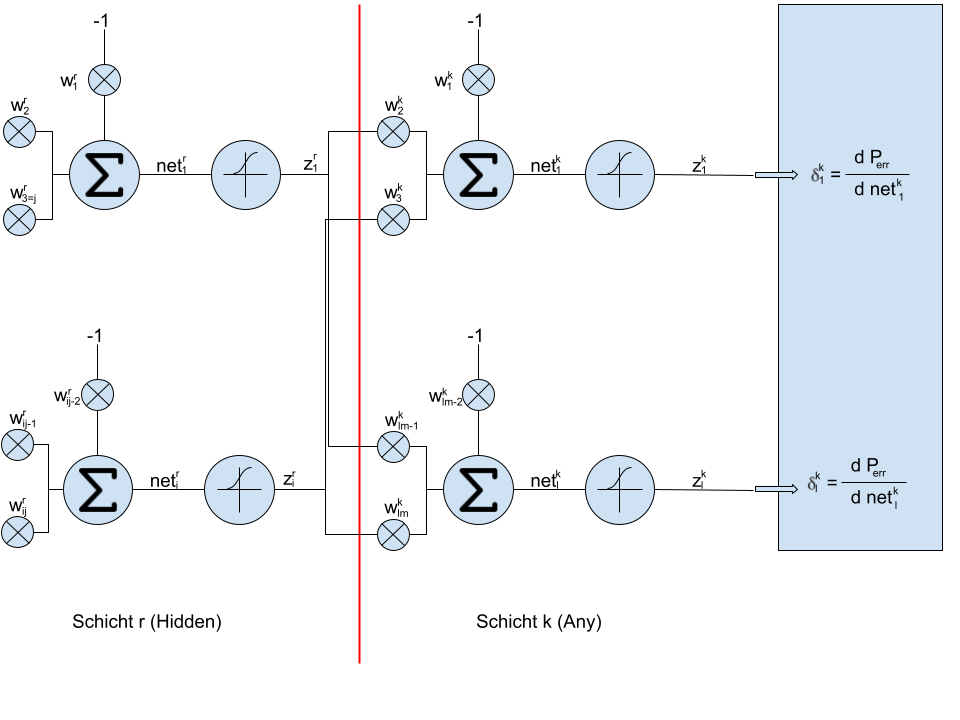
\includegraphics[width=1\linewidth]{../common/01_neuronal_network/00_resources/05_backpropagation_hidden.png}
    \end{center}
    \caption{Backpropagation für Hidden-Layer}
    \label{fig:09_backpropagation_hidden}
\end{figure}

Auch in diesem Fall geht es um die Berechnung des Terms $\delta_i^r$ in der grünen Ebene anhand der genannten bekannten Terme. Es müssen wiederum
alle Pfade, welche zu dem Neuron führen, betrachtet werden. Der Term $\delta_i^r$ setzt sich wie nachfolgend zusammen\footnote{Aus der Gleichung \ref{eq:05_delta_hidden}
ist ersichtlich, dass es sich bei $nm$ um den letzten Index aus den Neuronen handelt, wobei $n$
von $1$ bis $l$ läuft. Dieser Index führt immer über ein Gewicht $nm$ zu $z_i^r$. $m$ kann hier auch anders gewählt werden,
je nachdem, nach welchem $net^r$ abgeleitet werden soll.}:
\begin{align}
    \delta_1^k = \frac{\delta P_{err}}{\delta net_1^k}\\
    \delta_l^k = \frac{\delta P_{err}}{\delta net_l^k}\\
    \delta_i^r = \frac{\delta z_i^r}{\delta net_i^r} \cdot \delta_1^k \cdot w_{13}^k + \frac{\delta z_i^r}{\delta net_i^r} \cdot \delta_l^k \cdot w_{lm}^k\\
    \delta_i^r = \frac{\delta z_i^r}{\delta net_i^r} \cdot (\delta_1^k \cdot w_{13}^k + \delta_l^k \cdot w_{lm}^k)\\
    \delta_i^r = \frac{\delta z_i^r}{\delta net_i^r} \cdot \sum_n^l(\delta_n^k \cdot w_{nm}^k)\\
    \delta_i^r = z_i^r(1 - z_i^r) \cdot \sum_n^l(\delta_n^k \cdot w_{nm}^k)\label{eq:05_delta_hidden}
\end{align}
\\

Da der Term $\delta_i^r$ nun für beide Fälle bekannt ist, können zuletzt die Gewichte in der orangen Ebene korrigiert werden.
Man nehme an, dass es bei den Gewichten der Schicht $r$ die Inputs $z_{s}^{p}$ der vorherigen Schicht $p$ gibt.
In dem Fall lautet die Korrektur für $w_{ij}^r$:
\begin{align}
    \delta_i^r = \frac{\delta P_{err}}{\delta net_i^r}\\
    w_{ij, neu}^r = w_{ij, alt}^r + \lambda \cdot \delta_i^r \cdot \frac{net_i^r}{\delta w_{ij}^r}\\
    w_{ij, neu}^r = w_{ij, alt}^r + \lambda \cdot \delta_i^r \cdot z_{s}^{p}\label{eq:06_korrektur_gewicht_backpropagation}
\end{align}
Wichtig ist zu erkennen, dass dasjenige $z_s^p$ relevant ist, welches mit dem Gewicht $w_{ij}^r$ multipliziert wird.
In Bezug auf die beiden Abbildungen \ref{fig:08_backpropagation_output} und \ref{fig:09_backpropagation_hidden}
kann das Beispiel der orangen Ebene für $w_{ij}^r$ betrachtet werden. In dem Fall ist $z_s^p$ relevant. Im Falle des Gewichts
$w_{ij-2}^r$ führt der Weg über $-1$. Dieser Wert für den Bias könnte ebenso als Input $z_0^p$ der Schicht $p$ angesehen werden.
Damit ist \ref{eq:06_korrektur_gewicht_backpropagation} allgemeingültig.
\\

Zu guter Letzt kann noch der abschliessende Algorithmus \ref{alg:00_backpropagation} angegeben werden unter der Voraussetzung,
dass der Biaswert $-1$ als Input $z_0^p$ gegeben wird.\\
\begin{algorithm}[H]
    \For{o = last downto 2}{
        \If {o == last}{
            \For{t = 1 to i}{
                \textcolor{BackpropGreen}{$\delta_t^o$} $= $ \textcolor{BackpropBlue}{$(d_t^o - z_t^o)$} $\cdot z_t^o(1 - z_t^o)$
            }
        }
        \Else{
            \For{t = 1 to i}{
                \textcolor{BackpropGreen}{$\delta_t^o$} $= z_t^o(1 - z_t^o) \cdot \sum_n^l($ \textcolor{BackpropBlue}{$\delta_n^{o + 1}$} $\cdot w_{nm}^{o + 1})$
            }
        }
        \For{(t, h) = (1,1) to (i, j)}{
            \textcolor{BackpropOrange}{$\delta w_{th}^o$} $= \delta_t^o \cdot z_{h-1}^{o - 1}$\\
            $w_{th, neu}^o = w_{th, alt}^o + \lambda \cdot \delta w_{th}^o$
        }
    }
    \caption{Backpropagation Algorithmus}
    \label{alg:00_backpropagation}
\end{algorithm}
Hierbei gibt $o$ die zu berechnende Schicht an. Diese beginnt am Ende, also beim Output-Layer. Der Input-Layer wird nicht
berücksichtigt, weswegen das Verfahren bei der vorletzten Schicht stoppt.

\newpage
\subsection{XOR und die Lösung}
Um noch ein Beispiel einer nichtlinearen Funktion, welche ein neuronales Netz darstellt, zu nennen, wird das vorherige
Beispiel von \glqq XOR\grqq{} aus Kapitel \ref{chapter:02_xor_perceptron} wiederaufgegriffen. Diesmal wird ein neuronales Netz mit
zwei Inputs, einem Hidden-Layer mit zwei Neuronen sowie einem Output-Layer mit einem Neuron erstellt (siehe Abbildung
\ref{fig:10_xor_neuronal_network}).
\begin{figure}[h!]
    \begin{center}
        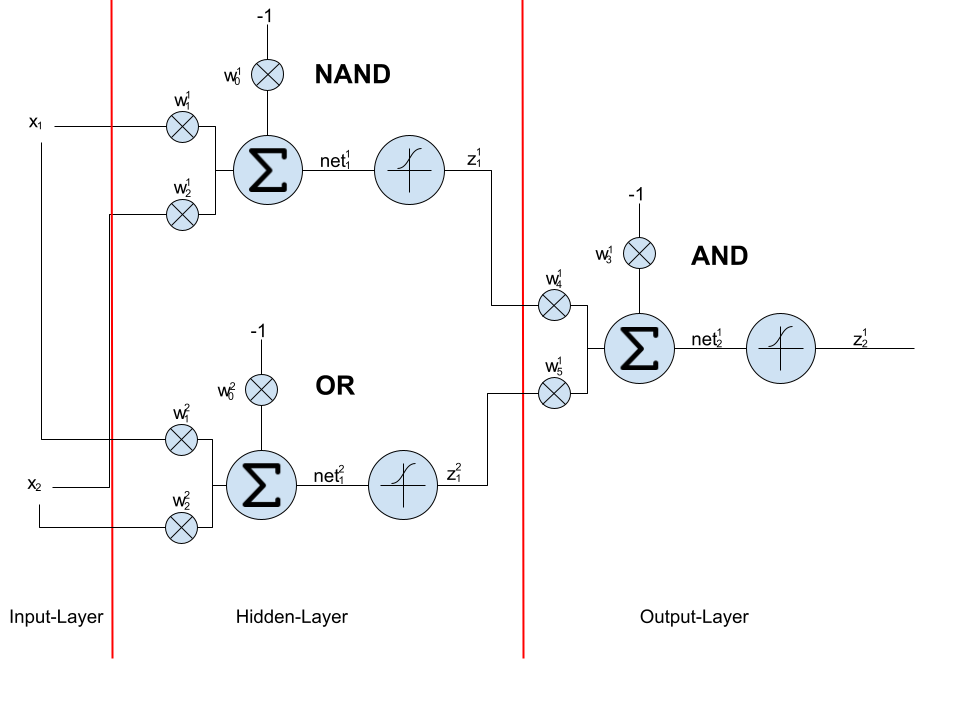
\includegraphics[width=1\linewidth]{../common/01_neuronal_network/00_resources/06_xor_neuronal_network.png}
    \end{center}
    \caption{Ein neuronales Netz für XOR}
    \label{fig:10_xor_neuronal_network}
\end{figure}
\newpage

Hierbei werden die Neuronen der Schichten speziell trainiert. Wie man in der Abbildung \ref{fig:11_xor_neuronal_network_operator}
entnehmen kann, ist \glqq XOR\grqq{} die Kombination durch \glqq AND\grqq{} von \glqq OR\grqq{} und \glqq NAND\grqq{}.
Diese Kombination wird ebenfalls durch das neuronale Netz in Abbildung \ref{fig:10_xor_neuronal_network} erzielt.
\begin{figure}[h!]
    \begin{center}
        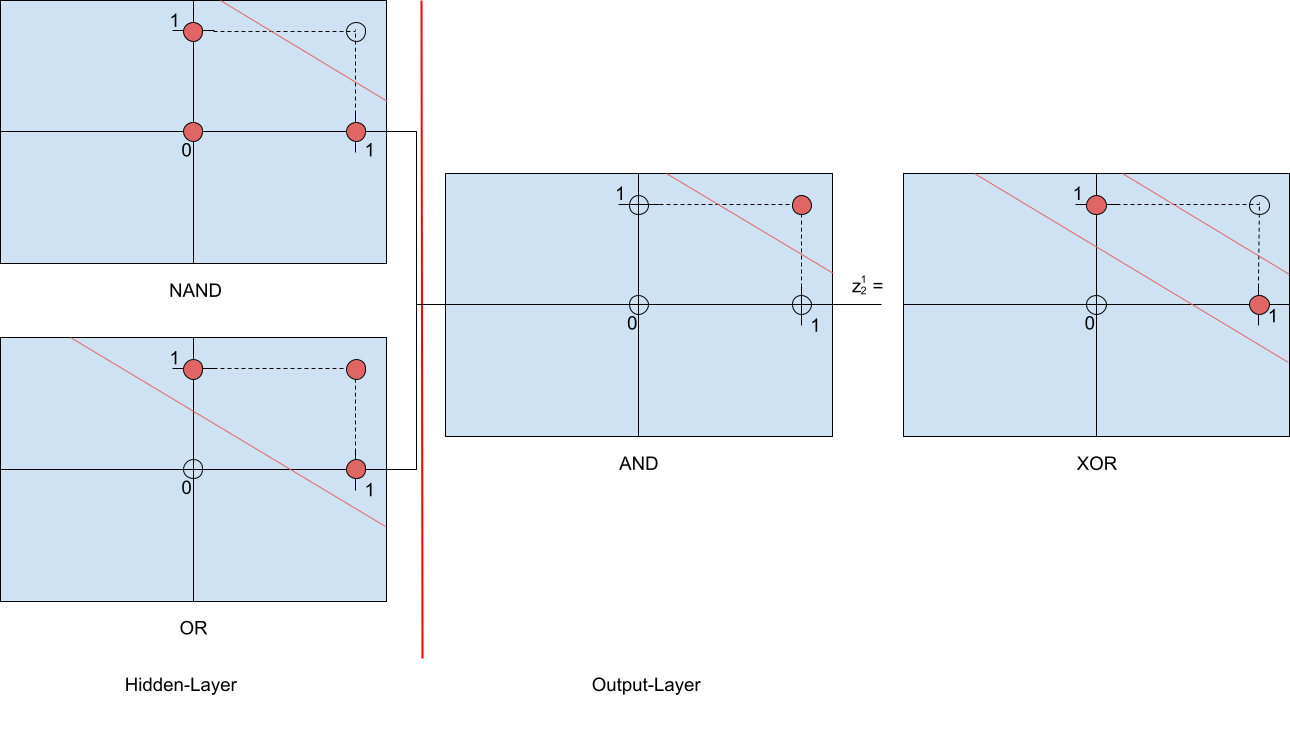
\includegraphics[width=1\linewidth]{../common/01_neuronal_network/00_resources/07_xor_neuronal_network_logical.png}
    \end{center}
    \caption{Die Kombination logischer Operatoren zur Erzielung von XOR}
    \label{fig:11_xor_neuronal_network_operator}
\end{figure}
\\

Mathematisch kann man sich ein \glqq XOR\grqq{} relativ gut vorstellen und dementsprechend die Architektur des neuronalen
Netzes wählen. Bei der Klassifikation in Bilderkennung ist dies jedoch nicht mehr so offensichtlich, weswegen beim Training des
Netzes auch sehr viele verschiedene Architekturen (Anzahl Hidden Layer, Anzahl Neuronen, usw.) ausprobiert werden müssen,
um eine möglichst gute Annäherung zu finden.